%! suppress = NonBreakingSpace
%! BibTeX Compiler = biber

% Preamble
\documentclass[12pt]{article}
\renewcommand{\baselinestretch}{1.5}
\author{Christoph Derszteler}

% Packages
\usepackage[T1]{fontenc}
\usepackage{lmodern}
\usepackage[utf8]{inputenc}
\usepackage[ngerman]{babel}
\usepackage[
  left=4cm,
  right=3cm,
  top=3cm,
  bottom=3cm
]{geometry}
\usepackage[bottom]{footmisc}
\usepackage{blindtext}
\usepackage{float}
\interfootnotelinepenalty=100000

\usepackage[hidelinks]{hyperref}
\hypersetup{
  linkcolor=black,
  linktoc=all,
}

\usepackage[
  citestyle=alphabetic,
  bibstyle=alphabetic
]{biblatex}
\DeclareCiteCommand{\footcite}[\mkbibfootnote]
{\usebibmacro{prenote}}
{\usebibmacro{citeindex}%
\printtext[brackets]{\usebibmacro{cite}}}
{\multicitedelim}
{\usebibmacro{postnote}}
\addbibresource{sources.bib}

\usepackage{graphicx}
\usepackage{booktabs}
\usepackage{gensymb}
\usepackage{siunitx}
\usepackage{amsfonts}
\usepackage{amsmath}
\usepackage{amssymb}
\usepackage{xcolor}
\usepackage{tikz}
\sisetup{
  group-separator = {,},
  input-decimal-markers={,},
  output-decimal-marker = {,},
  exponent-product={\ensuremath{\cdot}}
}

\counterwithin*{equation}{section}
\counterwithin*{figure}{section}
\renewcommand{\theequation}{\arabic{section}.\arabic{equation}}
\renewcommand{\thefigure}{\arabic{section}.\arabic{figure}}
\renewcommand{\thetable}{\arabic{section}.\arabic{table}}

\usepackage{tocloft}
\renewcommand{\cftpartleader}{\cftdotfill{\cftdotsep}}
\renewcommand{\cftsecleader}{\cftdotfill{\cftdotsep}}

\newcommand{\sectiontitle}{}
\newcommand{\newsection}[2]{\renewcommand{\sectiontitle}{#1}\section{#1}\label{sec:#2}}

\usepackage{fancyhdr}
\fancypagestyle{table-of-contents}{
  \fancyhead{}
  \chead{INHALTSVERZEICHNIS}
  \rhead{\thepage}
  \fancyfoot{}
  \renewcommand{\headrulewidth}{0.4pt}
}
\fancypagestyle{appendix}{
  \fancyhead{}
  \lhead{A}
  \chead{ANHANG}
  \rhead{\thepage}
  \fancyfoot{}
  \renewcommand{\headrulewidth}{0.4pt}
}
\pagestyle{fancy}
\lhead{\thesubsection}
\chead{\MakeUppercase{\sectiontitle}}
\rhead{\thepage}
\fancyfoot{}
\renewcommand{\headrulewidth}{0.4pt}

\usepackage{listings}
\usepackage{color}
\AtBeginDocument{
  \renewcommand{\lstlistingname}{Code}
  \renewcommand{\thelstlisting}{A.\arabic{lstlisting}}
}
\definecolor{mygreen}{rgb}{0, 0.6, 0}
\definecolor{mymauve}{rgb}{0.58, 0, 0.82}

% Document
\begin{document}
  \begin{titlepage}
  \begin{center}
    \vspace{1cm}

    Heinrich-Böll-Gymnasium Troisdorf\\
    Schuljahr 2022/2023

    \vspace{1cm}
    \Huge
    \line(1,0){400}\\
    \textbf{Die mathematischen Grundlagen der Mandelbrot-Menge}\\
    \line(1,0){300}\\

    \vspace{0.75cm}
    \Large
    und deren visuelle Darstellung mithilfe von Computerprogrammen

    \vspace{2cm}
    \large
    verfasst von\\
    \Large
    \textbf{Christoph Derszteler}

    \vfill
    \large
    Leistungskurs Mathematik\\
    Betreuer: Frau Dammers\\
    Abgabetermin: 23.02.2022 12:00 Uhr CET\\
  \end{center}
\end{titlepage}
  \newpage

  \tableofcontents{\thispagestyle{table-of-contents}}

  \newsection{Einleitung}{introduction}

Die Mandelbrot-Menge ist durch ihre hübschen, ansehnlichen Darstellungen verglichen
mit anderen mathematischen Phänomenen recht bekannt.
Dies liegt jedoch nicht nur an ihrer rein visuellen Attraktivität,
sondern vielmehr auch an Benoît Mandelbrot\hyperref[app:3]{[A.3]},
dem Entdecker dieser Menge.
Dieser sorgte mit seinen vielen Vorträgen und Büchern dafür, dass sich Fraktale,
also selbstähnliche\footnote{
  Das heißt, sich selbst wiederholend oder in ähnlicher Form erneut aufkommend.
}, geometrische Figuren mit gebrochener Dimension\footnote{
  Im Vergleich zu zum Beispiel einem zwei-dimensionalen Viereck.
}, vornehmlich die Mandelbrot-Menge, in der Bevölkerung weit verbreiteten
~\footcite[Vgl. letzten Absatz]{ibm_fractal_2011}.

Obwohl die Natur mit ihren fraktal-ähnlichen Formationen wie dem Aufbau einer
Schneeflocke, dem Verlauf eines Flusses oder die Verteilung von Baumästen
~\cite{nnart_fractals_nodate} die Inspiration für Mandelbrot war
~\cite{zink_kosmische_2014}, so liegt der Ursprung dieser Arbeit in den für
manchen simpler erscheinenden, viel moderneren aber dennoch genauso spannenden,
computer-generierten Videos\footcite[Vgl. bspw.][]{maths_town_eye_2017},
die man im Internet finden kann.
Mit unter anderem der Frage, wie diese Videos in Ansätzen generiert werden können
und vielem weiteren beschäftigt sich diese Arbeit.

Dafür jedoch und zum vollen Verständnis der Mandelbrot-Menge ist Grundlagenwissen
gewisser Themengebiete erforderlich, das in Kapitel 2 näher erörtert wird.
Kapitel 3 beschäftigt sich daraufhin mit der Mandelbrot-Menge selbst und insbesondere
mit der Analyse visueller Darstellungen dieser.
Abschließend befasst sich diese Arbeit in Kapitel 4 mit der praktischen Anwendung
der Mandelbrot-Menge in Form von Bildgenerierungen mithilfe von Computern als auch
anderweitigen Zusammenhänge zwischen dem theoretischen, mathematischen Konzept
der Mandelbrot-Menge und der realen Welt.

  \newsection{Theoretische Grundlage}{theoretical-foundation}

Die von Benoît Mandelbrot \hyperref[app:4]{[A.4]} entdeckte und nach ihm benannte
Mandelbrot-Menge befasst sich mit der bereits im vorherigen Kapitel vorgestellen,
komplexen Iteration \(z_{n+1} = z_n^2 + c \text{ mit } z_0 = 0\) und einem variablen
Wert für \(c\)~\cite*[S.25]{schuh_fraktale_2017}.
Die Mandelbrot-Menge enthält dabei alle Werte dieser Iteration, die beschränkt sind.
Mathematisch wird die Menge wie folgt definiert:

\[
  \mathbb{M} = \{c \in \mathbb{C} \; |\;  \forall n \in \mathbb{N}:\; |f_c^n(z)|\; \leqslant 2;\, n \to \infty\}
  \quad
  \text{mit}
  \quad
  f_c(z) = z^2 + c;\, z,c \in \mathbb{C}
\]
  \newsection{Mathematische Betrachtung}{mathematical-consideration}

Nachdem im vorherigen Kapitel die Grundlagen für die Mandelbrot-Menge
erklärt wurden, befasst sich diese Kapitel mit der rein mathematischen Betrachtung
dieser Menge, indem diese zunächst fachlich korrekt definiert und
im Anschluss grafisch analysiert wird.

\subsection{Mathematische Definition}\label{subsec:mathematical-definition}

Die Mandelbrot-Menge wird mit der bereits im vorherigen Kapitel vorgestellen,
komplexen Iteration $z_{n+1} = z_n^2 + c \text{ mit } z_0 = 0$ und einem variablen
% TODO: Update cite to new book
Wert für $c$~\cite*[S.25]{schuh_fraktale_2017} definiert.
Dabei enthält die Menge alle komplexen Werte für $c$, mit denen die
oben angegebene Iteration beschränkt ist.
Mathematisch ist die Menge iterativ wie folgt definiert:

\begin{equation}\label{eq:mathematical-definition}
  \mathbb{M} = \{c \in \mathbb{C} \; |\;  \forall n \in \mathbb{N}:\; |f_c^n(z)|\; \leqslant 2\}
  \quad
  \text{mit}
  \quad
  f_c(z) = z^2 + c;\, z,c \in \mathbb{C}
\end{equation}

Wie in der Definition zu sehen, wird der Funktionswert der
gegen Unendlich strebenden $n$-ten Iteration, ausgedrückt durch $f^n(z)$,
absolut betrachtet, was bedeutet, dass die Funktion symmetrisch zur reellen Achse ist.

Ebenfalls zu betrachten ist die Einschränkung auf Funktionswerte $\leqslant 2$, denn
für alle Funktionswerte, die sich in der oben genannten Iteration ergeben
und $> 2$ sind, lässt sich das jeweilige $c$ aus der Mandelbrot-Menge
ausschließen.
Obwohl der gesamte Beweis dessen über den Rahmen dieser Arbeit hinausginge,
so soll dennoch angemerkt werden, dass mithilfe der Dreiecksungleichung und
vollständiger Induktion unter der Vorausnahme von $|z_n| > 2 \text{ und } |z_n| > |c|$
folgende Ungleichung, die eine divergente Entwicklung repräsentiert,
$\frac{|z_{n+11}|}{|z_n|} > 1$ bewiesen werden kann~\cite{munafo_escape_1997},
wobei sich zusätzlich zeigen lässt, dass für alle Werte von $|c| > 2$
nach spätestens 2 Iterationen gilt: $z_{n=2} = |c^2 + c| \geqslant |c|^2 - |c| > 2$.

Es befinden sich deshalb alle Werte für $c$ als auch somit die grafische Darstellung
der Mandelbrot-Menge in einem Einheitskreis mit dem Radius 2 \hyperref[app:4]{[Vgl. A.4]}.
\subsection{Grafische Analyse}\label{subsec:graphical-analysis}

Im Folgenden soll der grundlegende Aufbau der in einem kartesischen Diagramm
entstehenden Formation der Mandelbrot-Menge erörtert als auch eine
Erklärung zur Farbbedeutung gegeben werden.
Zusätzlich zeigt dieses Unterkapitel mit einer exemplarischen Kartografierung
verschiedene, sich wiederholende Bereiche der visuellen Darstellung auf.

\begin{figure}[h!]
  \centering
  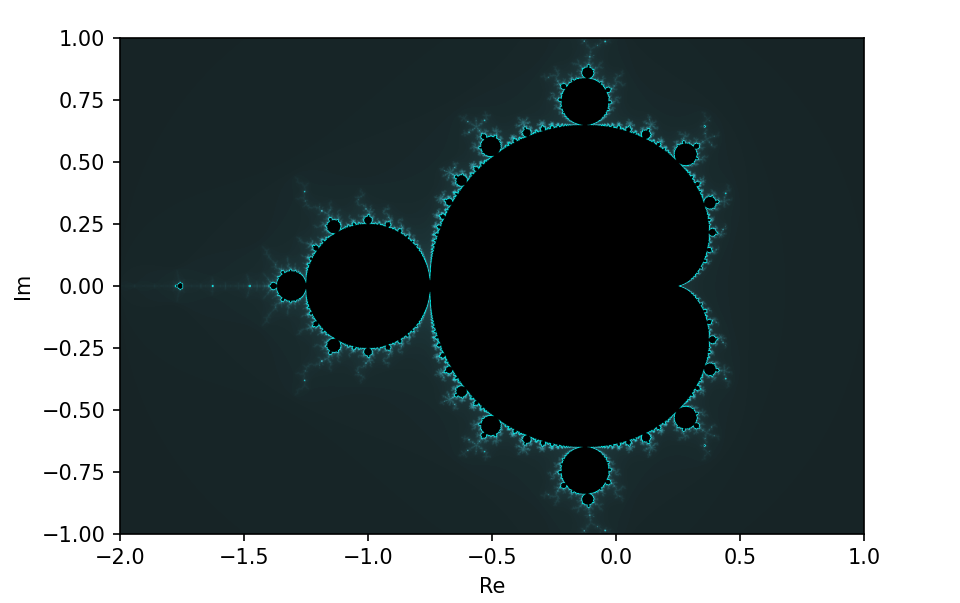
\includegraphics[width=\textwidth]{images/mandelbrotImage}
  \caption[Caption for LOF]{
    Exemplarische Darstellung der Mandelbrot-Menge\footnotemark
  }
  \label{fig:mandelbrot-set}
\end{figure}
% TODO: Fix clickable
\footnotetext{
  Generiert durch den Code \hyperref[app:last]{A.Last} mit eint einer
  \glqq RESOLUTION\grqq~von $2000$ und einer \glqq MAX\_ITERATIONS\grqq~von $500$
}

Die hier zu sehende Grafik entspricht der Darstellung der Mandelbrot-Menge
in einer komplexen Zahlenebene und wird aufgrund seiner Form
\glqq Apfelm\"annchen\grqq~genannt.
Die zu sehenden, schwarz gefärbten Pixel repräsentieren einen
jeweiligen Wert für $c$, der sich in der Mandelbrot-Menge befindet.
Auffällig ist bei erster Betrachtung, dass sich neben der großen,
einheitlichen Struktur in der Mitte,
deutlich kleinere, ähnlich aussende Formationen um den eigentlichen Hauptkörper
dem Apfelm\"anchen, zum Beispiel im negativen Teil der reellen Achse,
erkennen lassen.
Diese werden \textbf{Satelliten} genannt und existieren aufgrund der Selbstähnlichkeit
der Mandelbrot-Menge in unendlicher Stückzahl - und zwar nicht nur für den Hauptkörper,
sondern auch für jeden Satelliten selbst~\cite{lomonaco_quasi-conformal_2018}.

\subsubsection{Farbbedeutung}\label{subsubsec:color-meaning}

Im Gegensatz zu den ersten grafischen Darstellungen der Mandelbrot-Menge,
auf denen, aufgrund ihrer deutlich geringeren Auflösung,
kleine Satelliten als Druckfehler gewertet wurden\footnote{
  Dies ist eine recht amüsante Anekdote: Während den frühsten Forschungen,
  die Benoît Mandelbrot in den 1970er bei IBM anstellte, war das Drucken deutlich
  mühseliger und aufwendiger, als es heutzutage ist.
  Deshalb existierte ein ganzes Abteil nur für die Herstellung und Bearbeitung von
  Drucks, die - da es damals häufig vorkam - kleine Satelliten am Rande der ersten
  Darstellungen \hyperref[app:5]{[A.5]} gutgemeint wegretuschierten.
  Die ersten Bilder, die Herr Mandelbrot also erhielt, verwunderten ihn sehr und
  er war äußerst aufgebracht, als er von der tolpatschigen Wahrheit erfur
  \cite{numberphile_whats_2019}.
}
und die mit ihrem schwarz-weißen Druck nur zwischen Werte für $c$ \textbf{in}
und \textbf{außerhalb} der Mandelbrot-Menge unterschieden,
besitzt die oben dargestellte
\hyperref[fig:mandelbrot-set]{Figur (\ref{fig:mandelbrot-set})}
einen Farbverlauf.
Dieser, in diesem Fall türkisblaue, Farbgradient gibt an,
wie viele Iterationen es benötigte,
um festzustellen, ob das jeweilige $c$ außerhalb der Mandelbrot-Menge liegt.
Dabei gilt, dass je heller der Pixel beziehungsweise $c$ ist, desto mehr
Iterationen hat es benötigt, um $c$ aus $\mathbb{M}$ auszuschließen\footnote{
  Vgl. z.B. dick markierten Werte für $c_1 = 1 \text{ und } c_3 = 0.5$ in
  \hyperref[tab:iterations-example]{Tabelle~\ref{tab:iterations-example}}.
  $c_1$ ließ sich nach der 3. Iteration aus der Mandelbrot-Menge ausschließen,
  hingegen war dies bei $c_3$ erst nach der 5. Iteration der Fall.
}.
Deshalb existiert ein hell erscheinender Rand um die schwarzen Formationen,
da es für diese Werte außerhalb von $\mathbb{M}$, die sehr nah an tatsächlichen
Werten für $\mathbb{M}$ sind, es viele Iterationen benötigt, um diese auszuschließen.

Neben dieser einen, verhältnismäßig simplen und dementsprechend auf den ersten
Blick aussagekräftigeren Farbkodierung, existiert eine Vielzahl teils deutlich
umfangreicheren Algorithmen, mit denen sich jedoch eine auf das menschliche Auge
ansprechendere Farbgestaltung erzielen lässt.
Diese werden in der \hyperref[subsubsec:color-coding]{Sektion \ref{subsubsec:color-coding}}
genauer beschrieben.
Eine Reihe an solchen komplexere Farbverläufe benutzenden Beispielen,
auf die im nächsten Unterkapitel Bezug genommen wird,
lässt sich in \hyperref[app:6]{A.6} betrachten.

\subsubsection{Exemplarische Kartografierung}

Die hingegen von der Farbe unabhängigen, entstehenden Formationen der
Mandelbrot-Menge, die teilweise erst bei sehr kleinen Ausschnitten erkennbar sind,
sind kartografiert und teilweise, wegen einer gewissen Ähnlichkeit, nach
Objekten aus der realen Welt benannt.
So bezeichnet man die größte kreisförmige Kardioide oder auch \glqq Knospe\grqq
~als \glqq K\"orper\grqq~(wobei dieser genauer unterteilt werden kann)
und die daran angrenzende Kardioide als
\glqq Kopf\grqq\footnote{Vgl. \hyperref[app:7]{A.7}}.

Obwohl man jeden Punkt beziehungsweise jeden Ausschnitt einzeln beliebig detailliert
analysieren kann, werden aufgrund der Selbstähnlichkeit Elemente mit ähnlichem
oder gleichen Aufbau erneut aufkehren und dementsprechend gleich benannt.
Im Folgenden soll beispielhaft ein Ausschnitt des in diesem
Video~\cite{beyer_zoomfahrt_2017} gezeigten
\glqq Tal der Seepferdchen\grqq~analysiert werden:

Die Spalte zwischen Kopf und K\"orper wird \glqq Tal der Seepferdchen\grqq
~genannt\footnote{Vgl. \hyperref[app:6.1]{A.6.1}}
~\cite{robert_p_seahorse_2010}, da bei Vergrößerung dieses Ausschnitts
sich unter anschaulicher Farbkodierung auf der rechten Seite
Seepferdchen-ähnliche Formationen erkennen lassen\footnote{Vgl. \hyperref[app:6.2]{A.6.2}}.
Vergrößert man die Sicht auf das Seepferdchen-Tal stark, so lassen sich,
neben weiteren (teils deformierten) Satelliten\footnote{Vgl. \hyperref[app:6.3]{A.6.3}},
bei genauerer Betrachtung des \glqq Seepferdchenschwanzes\grqq~ein
Misiurewicz-Punkt erkennen\footnote{Vgl. \hyperref[app:6.4]{A.6.4}}.
Dieser Misiurewicz-Punkt zeigt ebenfalls die Selbstähnlichkeit der Mandelbrot-Menge auf,
da dieser Punkt sich neben einer Drehung kaum von der eigentlichen
Mandelbrot-Menge unterscheidet~\cite{lei_similarity_1989}.
Vergrößert man diesen Punkt weiter, so findet man erneut einen im Vergleich
zum Apfelm\"annchen sehr ähnlichen aussehenden
Satelliten\footnote{Vgl. \hyperref[app:6.5]{A.6.5}}.
  \newsection{Praktische Anwendung}{practical-application}

Im Folgenden werden die im letzten Kapitel untersuchten mathematischen Betrachtungen
unter Realbedingungen angewandt, indem die dadurch entstehenden Grenzen
spezifiziert als auch die konkreten Umsetzungen exemplarisch dargestellt werden.
Dafür beschäftigt sich diese Arbeit zunächst mit der informationstechnischen
Herangehensweise zur Generierung bereits dargestellter Bilder.
Darauffolgend sollen zusätzliche Informationen zu anderweitigen mit der
Mandelbrot-Menge in Verbindung stehenden Phänomen gegeben werden.

\subsection{Digitale Bildgenerierung}\label{subsec:digital-generation}

Im weiteren Verlauf werden informationstechnische Aspekte
hinsichtlich der Bildgenerierung der Mandelbrot-Menge untersucht.
Dafür werden zunächst die Funktionsweise als auch die dabei durch die Unterschiede
zur reinen Mathematik entstehenden Probleme erläutert.
Im Anschluss werden verschiedene Herangehensweisen und Algorithmen zur Farbkodierung
exemplarisch vorgestellt.

\subsubsection{Korrelation zwischen Informationstechnik und Mathematik}
\label{subsubsec:correlation-between-it-and-mathematics}

Die im letzten Kapitel analysierte \hyperref[fig:mandelbrot-set]
{Abbildung \ref{fig:mandelbrot-set}} wurde,
wie in der Beschriftung beschrieben, mit dem Code aus \hyperref[app:10]{A.10}
generiert.
Im Vergleich zu den mathematischen Überlegungen ist die
informationstechnische Herangehensweise dabei sehr ähnlich:

Grundlegend wird jeder Pixel mit seiner $x$- und $y$-Koordinate des zu generierenden
Ausschnitts einer komplexen Zahl zugeordnet.
Dabei entspricht (in der regulären Darstellung) die $x$-Koordinate dem Realteil
$a$ und die $y$-Koordinate dem Imaginärteil $b$, sodass eine komplexe Zahl
$z = a + bi$ in einem Pixel $P \text{ durch } x = a \text{ und } y = b$ ausgedrückt
werden kann.

Das naheliegendste Problem, neben vielen ausschließlich informationstechnischen
Optimierungsaufgaben, ergibt sich bei der Berechnung, ob es sich beim jeweiligen Pixel
beziehungsweise dem jeweiligen $c$, um ein Element in
$\mathbb{M}$ handelt.
Denn im Gegensatz zu der mathematischen Betrachtung ist es in der konkreten Umsetzung
nicht möglich, die Iterationsanzahl $n$ bei $f^n(z)$ gegen Unendlich konvergieren zu lassen.
Deshalb setzt man einen Grenzwert $m$ an Iterationsdurchläufen, ab dem,
sofern das zu überprüfende $c$ noch nicht aus der Mandelbrot-Menge
ausgeschlossen wurde, dieses als Element von $\mathbb{M}$ angenommen wird.

Folglich bestimmt dieser Wert indirekt die Auflösung beziehungsweise Genauigkeit
des zu generierenden Bilds und muss deshalb bei kleineren Ausschnitten besonders
hoch sein, da dabei ein Unterschied zwischen komplexen Zahlen ausgemacht werden
muss, dessen Werte sich lediglich um geringe Nachkommastellen unterscheiden.
Die Auswirkungen dieser Iterationsgrenze sind durch die Bildergalerie
\hyperref[app:8]{A.8}, die generierte Bilder der Mandelbrot-Menge
mit unterschiedlich (niedrigen) Grenzen darstellt, anschaulich visualisiert.

\subsubsection{Farbkodierung}\label{subsubsec:color-coding}

Um die in der \hyperref[subsubsec:color-meaning]{Sektion \ref{subsubsec:color-meaning}}
erklärten Farben zu kodieren, eignet sich zunächst das HSV (Hue, Saturation, Value)
Farbmodel, womit sich mithilfe von prozentualen Werten eine
Farbveränderung hinsichtlich sowohl der Helligkeit
als auch der Farbsättigung erzielen lässt.
Dies wird anhand des Verhältnisses der benötigten Iterationen $n$ zu der Iterationsgrenze $m$
für jeden zu überprüfenden komplexen Wert $c \text{ für } \mathbb{M}$
berechnet \cite{robert_p_color_2022}.
Als Beispiel sei Hue mit $186\degree$ und Value mit $100\%$ gegeben, woraus
sich für jedes $c$ folgendes HSV ergibt:
$ HSV(186\degree, \frac{n}{m} \cdot 100\%, 100\%)$.

Diese Farbkodierung ist aufgrund ihrer Simplizität in ihrer beschriebenen
Form direkt informationstechnisch umsetzbar, jedoch eignet sich solch eine
Herangehensweise aus Performance- beziehungsweise Optimierungsgründen nicht
für jede zu überprüfende, komplexe Zahl $c$, wenn es sich bei der
Farbzusammenstellung um einen komplexeren Zusammenhang wie in den Elementen
der Bildergalerie \hyperref[app:6]{A.6} handelt.
Um dieses Problem zu lösen, erstellt man sogenannte Colormaps
(engl.: Farbpaletten), wie zum Beispiel \hyperref[app:9.1]{\ref{app:9.1}}
aus den Werten des oberen Beispiels.
Für ein jeweiliges $c$ wird mithilfe solcher Farbpaletten eine Farbe erneut anhand
dessen Verhältnisses von benötigten Iterationen $n$ zu der Iterantionsgrenze $m$
ermittelt; dabei existieren jedoch bereits alle vorkommenden Farben, was somit
die Berechnung des aufwendigeren Farbgenerierungsprozesses\footnote{
  Also die Auswahl und korrekte Zusammenstellung der Farben einer Farbpalette.
}
von dem Berechnungsprozess der eigentlichen Mandelbrot-Menge entkoppelt.
In \hyperref[app:9.2]{\ref{app:9.2}} ist die für alle für die Arbeit generierten
Abbildungen benutzte Colormap zu sehen, die im Vergleich zur vorherigen
dargestellten Palette mehr als zwei (insgesamt 4) Ankerpunkte\footnote{
  Hier: Eindeutige HSV-Farben, die in gewissen Abständen auf einer Palette
  platziert werden und zwischen denen ein Gradient ensteht.
} besitzt, wobei diese, im Gegensatz zu einer komplexen\footnote{
  Eine Farbpalette mit vielen Ankerpunkten.
} Colormap \hyperref[app:9.3]{[z.B. \ref{app:9.3}]},
mit der man visuell anschaulichere Bilder generieren kann,
weiterhin recht minimal ist.
\subsection{Anderweitige Zusammenhänge}\label{subsec:other-connections}

Neben den bisher bereits mehrfach angesprochenen
\glqq Mandelbrot Videos\grqq\footnote{
  Auch unter \glqq Zoomvideos\grqq~oder \glqq Bilderfahrten\grqq~zu finden
}, die ebenfalls einen digitalen Zusammenhang zu der Mandelbrot-Menge besitzen
und die trotz ihres Primärziels, das normalerweise die Unterhaltung ist, eine
ausgesprochene Komplexität besonders hinsichtlich ihrer Optimierungsmöglichkeiten,
aufweisen, denen man problemlos eine eigene Arbeit dedizieren könnte,
gibt es, wie in der Einleitung erwähnt,
viele biologische Zusammenhänge zwischen der Natur und Fraktalen:
Obwohl es über den Umfang dieser Arbeit hinausgehen würde, auf diesen Bereich
der Biologie genauer einzugehen, so soll dennoch angemerkt werden,
dass Fraktale wie die Mandelbrot-Menge der Natur ermöglichen,
komplexe Anordnungen und Konstruktionen möglichst ressourcen- und platzschonend
darzustellen, da Informationen sowohl für beispielsweise den Baumstamm als auch
einen kleinen Ast aufgrund der, wie bei Satelliten der Mandelbrot-Menge auftretenden,
Selbstähnlichkeit von Fraktalen nur einmal gespeichert werden müssen.

  \newsection{Fazit}{conclusion}

Zusammenfassend lässt sich festhalten, dass durch die verhältnismäßig simple
Gleichung $z_{n+1} = z_n^2 + c$ sich eine riesige Welt der Fraktale eröffnet
hat, die durch ihre visuellen Darstellungen mit ihrer atemberaubenden Schönheit
nicht nur eine Nische an Mathematikern, sondern seit langem erneut auch die
breitere Gesellschaft erreichen und erstaunen konnte.
Diese Arbeit hat einen grundlegenden Überblick über die Mathematik hinter der
Mandelbrot-Menge geliefert als auch eine Erklärung und die damit einhergehenden
Komplikationen zur Generierung solcher faszinierenden Bildern dargelegt.

Nichtsdestotrotz ist der abgedeckte Bereich dieser Abhandlung begrenzt, denn es
existieren unzählige weitere Zusammenhänge zwischen der Mandelbrot-Menge und
anderen mathematischen Phänomenen wie Pi oder der Fibonacci-Folge.
Es würde sich ebenfalls nicht um eine vollständige Arbeit über die
Mandelbrot-Menge handeln, wenn nicht die Julia-Mengen und ihre enge Verknüpfung
zu der als übergeordnet zu betrachtenden Mandelbrot-Menge erwähnt werden würde.

Abschließend lässt sich jedoch nur sagen, dass man gespannt abwarten kann,
welche interessanten Entdeckungen diesem jungen Gebiet der Mathematik folgen werden.

  \newsection{Literatur und Quellen}{literature-and-sources}
  \nocite{heinrich_boll_gymnasium_troisdorf_hbg_nodate}
  \printbibliography[heading=none]
  \newpage

  \newsection{Selbstständigkeitserklärung}{declration-of-independence}

Hiermit erkläre ich, dass ich die Facharbeit selbstständig und ohne fremde Hilfe
angefertigt und nur die im Literaturverzeichnis angeführten Quellen und Hilfsmittel
benutzt habe.
Alle verwendeten Materialien habe ich im Anhang angegeben.
Ich erkläre ferner verbindlich, dass ich alle Zitate kenntlich gemacht habe
und ihre Herkunft im Anhang angeben habe.
Mir ist klar, dass ein Zuwiderhandeln gegen diese Bestimmungen zu einer
0-Punkte Bewertung der Arbeit führt.

\bigskip
\noindent
Niederkassel, den \hfill\underline{\hspace{4cm}}

\medskip
\noindent
Unterschrift des Verfassers: \hfill\underline{\hspace{4cm}}

  \newsection{Anhang}{appendix}
\newcommand{\figuretag}[1]{%
  \addtocounter{figure}{-1}%
  \renewcommand{\thefigure}{#1}%
}
\noindent\textbf{A.1:}\label{app:1}
\begin{equation}\tag{A.1}\label{eq:complex-numbers-multiplication}
  \begin{split}
    z_1 \cdot z_2 \\
    (a + bi) \cdot (c + di) \\
    =  c(a + bi) + di(a + bi) \\
    = ac + bci + adi + bdi^2 \\
    = ac + bci + adi \boldsymbol{ - } bd \\
    = ac - bd +(bc + ad)i
  \end{split}
\end{equation}

\noindent\textbf{A.2:}\label{app:2}
\begin{equation}\tag{A.2}\label{eq:complex-numbes-squaring}
  \begin{split}
    z_1^2
    = z_1 \cdot z_1 \\
    = (a + bi) \cdot (a + bi) \\
    = a \cdot (a + bi) + bi \cdot (a + bi) \\
    = a^2 + abi + abi - b^2 \\
    = a^2 - b^2 + 2abi
  \end{split}
\end{equation}

\noindent\textbf{A.3:}\label{app:3}
\begin{figure}[H]\figuretag{A.3}\label{fig:benoit-mandelbrot-picture}
\begin{center}
  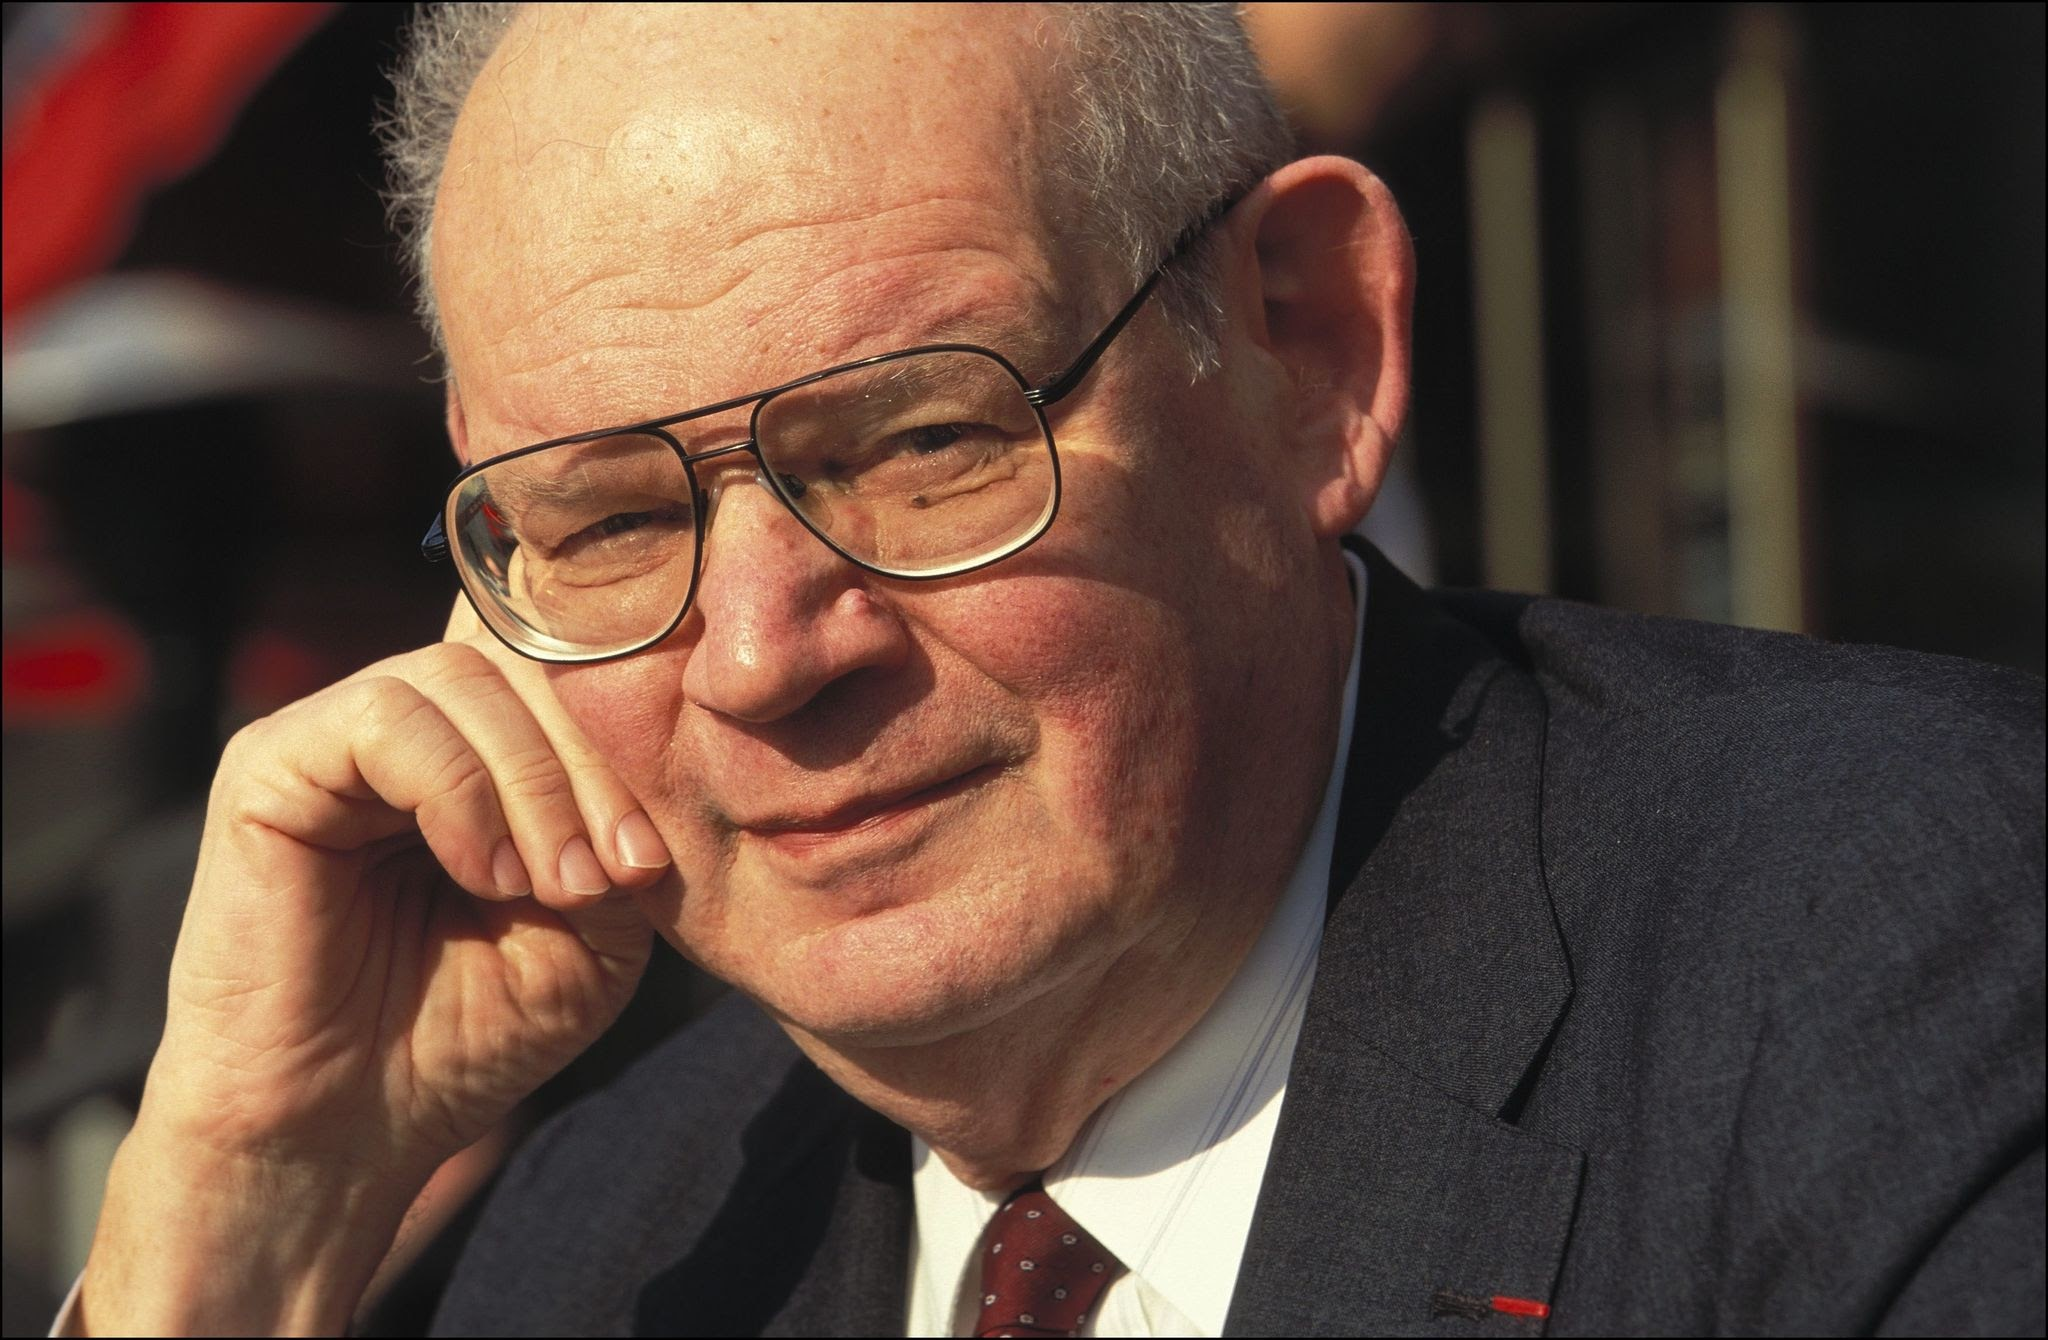
\includegraphics[width=0.7\textwidth]{images/benoit-mandelbrot}
  \caption{Benoît Mandelbrot 1997 in Frankreich~\cite{gaillarde_benoit_1997}.}
\end{center}
\end{figure}

\noindent\textbf{A.4:}\label{app:4}
\begin{figure}[H]\figuretag{A.4}\label{fig:escape-radius}
  \begin{center}
    \begin{tikzpicture}
      \begin{scope}[thick,font=\scriptsize]
        \fill[draw=black, fill=white] (0,0) circle (2);

        \draw [fill=black] (1,1.6) circle(0.05);
        \draw [fill=black] (-3,2.75) circle(0.05);
        \node at (1.75,1.85) {$ P_1(1|1.6i)$};
        \node at (-1.75,3) {$ P_2(-3|2.75i)$};

        \draw [->] (-4,0) -- (4,0) node [above left]  {$Re$};
        \draw [->] (0,-4) -- (0,4) node [below right] {$Im$};

        \foreach \n in {-3,...,-1,1,2,...,3}{
          \draw (\n, 3pt) -- (\n, -3pt)   node [below] {$\n$};
          \draw (3pt,\n) -- (-3pt,\n)   node [left] {$\n i$};
        }
      \end{scope}
    \end{tikzpicture}
    \caption{
      Einheitskreis mit dem Radius 2. Zu sehen ist der Punkt $P_1$, der im
      Einheitskreis liegt und Punkt $P_2$, der außerhalb des Einheitskreises liegt.
    }
  \end{center}
\end{figure}

\noindent\textbf{A.5:}\label{app:5}
\begin{figure}[H]\figuretag{A.5}\label{fig:body-and-head-of-mandelbrot-set}
\begin{center}
  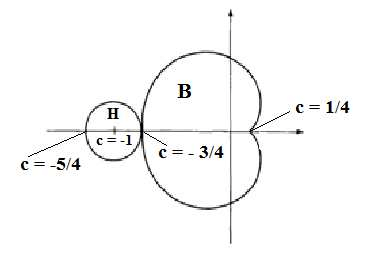
\includegraphics[width=0.7\textwidth]{images/bodyHeadMandelbrotSet}
  \caption{
    K\"orper (B) und Kopf (H) der Mandelbrot-Menge~\cite{mahanta_mandelbrot_2016}.
  }
\end{center}
\end{figure}

\noindent\textbf{A.6:}\label{app:6}
\begin{figure}[H]\figuretag{A.6}\label{fig:mandelbrot-set-zoom-images}
  \centering
  \begin{minipage}[t]{0.40\textwidth}
    \centering
    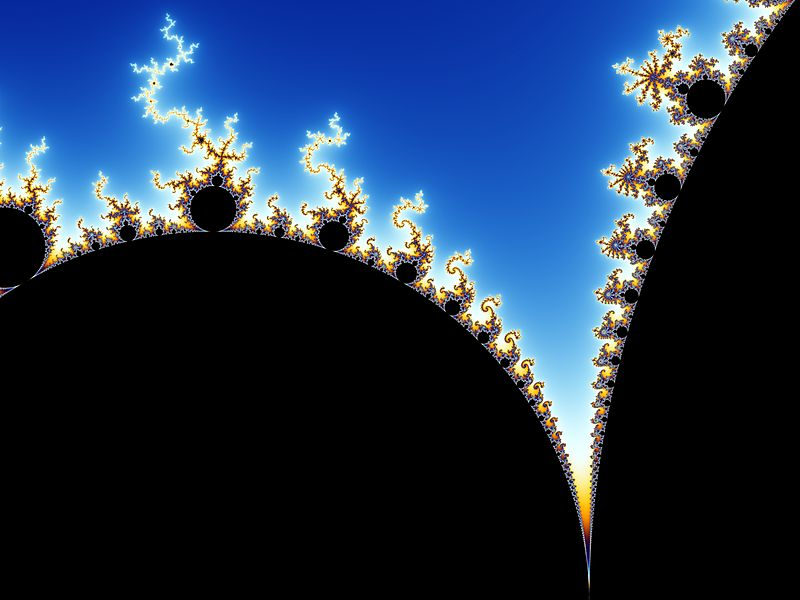
\includegraphics[width=\linewidth]{images/zoom/800px-Mandel_zoom_01_head_and_shoulder}
    \figuretag{A.6.1}
    \vspace*{-4ex}
    \caption{Spalte zwischen Kopf und K\"orper~\cite{beyer_partial_2005}}
    \label{app:6.1}
  \end{minipage}%
  \hspace{8ex}
  \begin{minipage}[t]{0.40\textwidth}
    \centering
    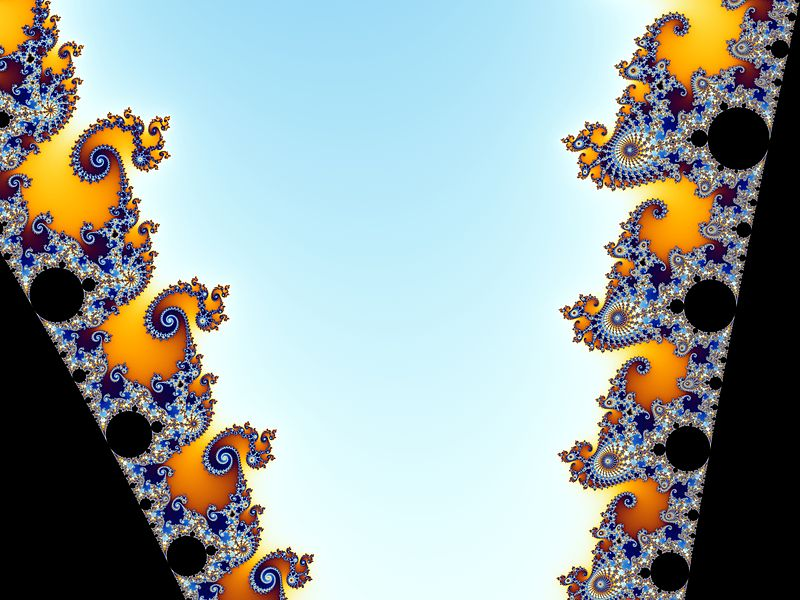
\includegraphics[width=\linewidth]{images/zoom/800px-Mandel_zoom_02_seehorse_valley}
    \figuretag{A.6.2}
    \vspace*{-4ex}
    \caption{\grqq Tal der Seepferdchen\glqq~\cite{beyer_partial_2005-1}}
    \label{app:6.2}
  \end{minipage}
  \\[4ex]
  \begin{minipage}[t]{0.40\textwidth}
    \centering
    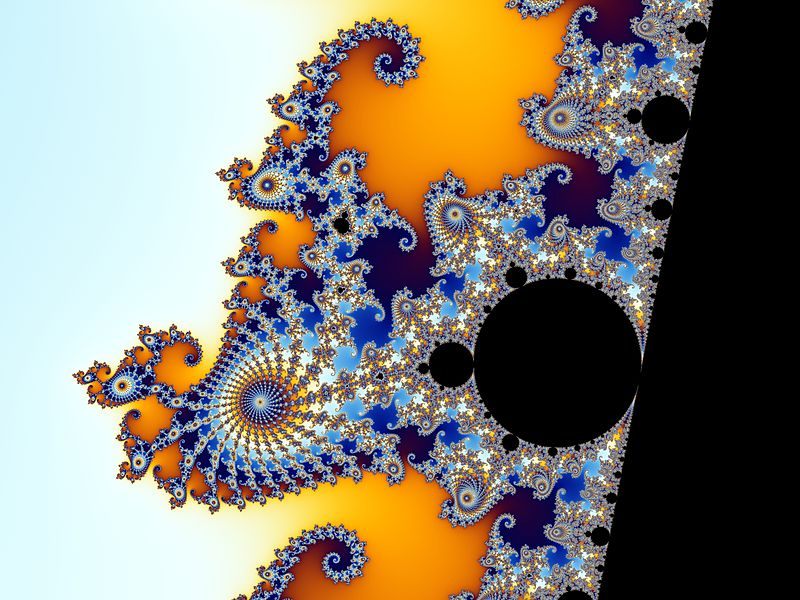
\includegraphics[width=\linewidth]{images/zoom/800px-Mandel_zoom_03_seehorse}
    \figuretag{A.6.3}
    \vspace*{-4ex}
    \caption{Rechts ein deformierter Satellit und links Misiurewicz-Punkt~\cite{beyer_partial_2005-2}}
    \label{app:6.3}
  \end{minipage}%
  \hspace{8ex}
  \begin{minipage}[t]{0.40\textwidth}
    \centering
    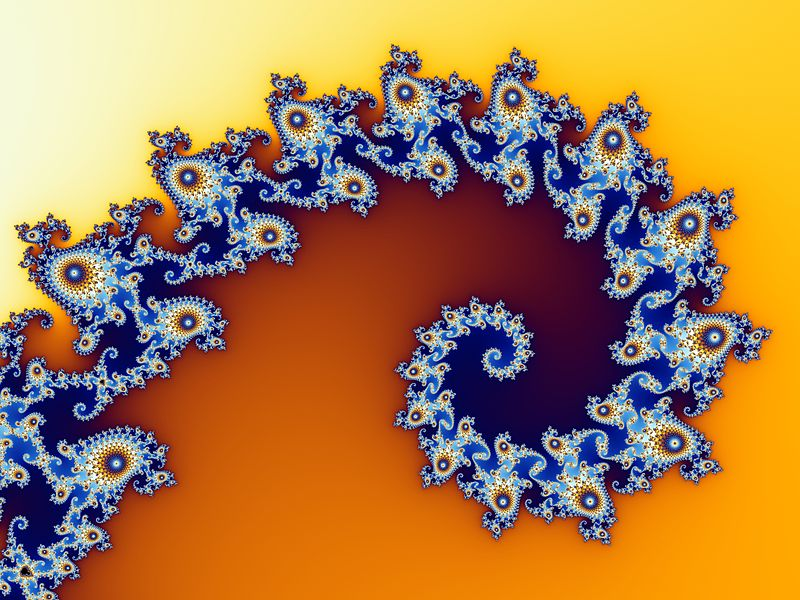
\includegraphics[width=\linewidth]{images/zoom/800px-Mandel_zoom_04_seehorse_tail}
    \figuretag{A.6.4}
    \vspace*{-4ex}
    \caption{Misiurewicz-Punkt~\cite{beyer_partial_2005-3}}
    \label{app:6.4}
  \end{minipage}
  \\[4ex]
  \begin{minipage}[t]{\textwidth}
    \centering
    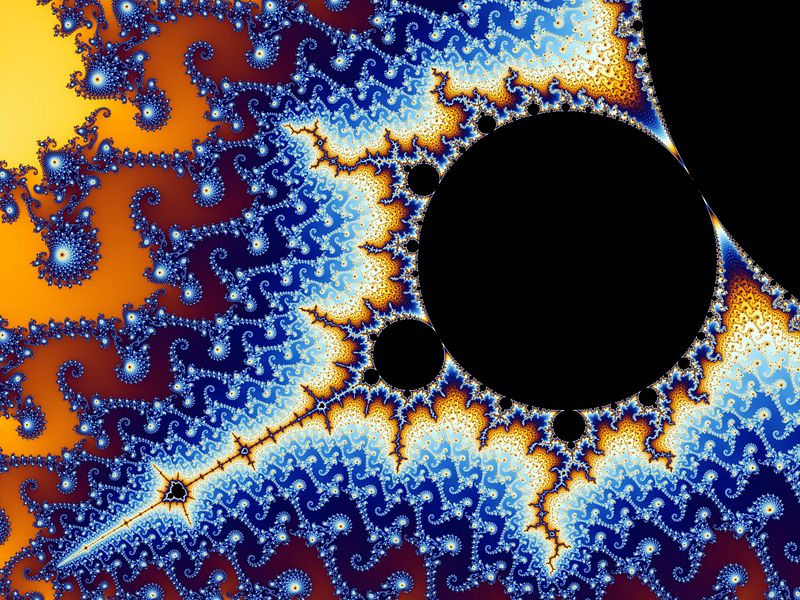
\includegraphics[width=0.45\linewidth]{images/zoom/800px-Mandel_zoom_08_satellite_antenna}
    \figuretag{A.6.5}
    \vspace*{-2ex}
    \caption{Satellit mit ähnlicher Struktur wie das Apfelm\"annchen~\cite{beyer_partial_2005-4}}
    \label{app:6.5}
  \end{minipage}
\end{figure}

\end{document}